\documentclass[a4paper, article, oneside, USenglish, IN5460]{memoir}

%% Title page
\usepackage{style/projectfp} 


%% Encoding
\usepackage[utf8]{inputenx} % Source code
\usepackage[T1]{fontenc}    % PDF


%% Fonts and typography
\usepackage{lmodern}           % Latin Modern Roman
\usepackage[scaled]{beramono}  % Bera Mono (Bitstream Vera Sans Mono)
\renewcommand{\sfdefault}{phv} % Helvetica
\usepackage[final]{microtype}  % Improved typography
\renewcommand{\abstractnamefont}{\sffamily\bfseries}                 % Abstract
\renewcommand*{\chaptitlefont}{\Large\bfseries\sffamily\raggedright} % Chapter
\setsecheadstyle{\large\bfseries\sffamily\raggedright}               % Section
\setsubsecheadstyle{\large\bfseries\sffamily\raggedright}            % Subsection
\setsubsubsecheadstyle{\normalsize\bfseries\sffamily\raggedright}    % Subsubsection
\setparaheadstyle{\normalsize\bfseries\sffamily\raggedright}         % Paragraph
\setsubparaheadstyle{\normalsize\bfseries\sffamily\raggedright}      % Subparagraph

%% Mathematics
\usepackage{amssymb}   % Extra symbols
\usepackage{amsthm}    % Theorem-like environments
\usepackage{thmtools}  % Theorem-like environments
\usepackage{mathtools} % Fonts and environments for mathematical formuale
\usepackage{mathrsfs}  % Script font with \mathscr{}
% Bibliography
\usepackage[backend=biber,style=numeric-comp]{biblatex}


\title{Appliance Energy Consumption Prediction and Classification Using Federated Learning}
\authors{F. Ofstad, Z. Shan, R. Syed, H. Zhang}

\addbibresource{bibliography.bib}

\begin{document}

\projectfrontpage


\chapter{Introduction}

The purpose of this report is to construct a Federated Learning model, which aggregates the resulting weights from client models. The client models have two tasks:
\begin{enumerate}
    \item to train a model to predict the energy consumption for appliances in a household
    \item Train a model to classify the type of appliance based on their energy consumption.    
\end{enumerate}

To this end, we used the tensorflow package for Python when creating the client models using Keras, and the extension tensorflow federated for the aggregating model. The steps the program takes are as follows. 


\section{Pre-processing the data}
We first convert the provided excel file into csv files for each household. This is done to conceptually emulate FL as each client should only have access to their own data, and because CSV files are generally faster to load in python.

Then for the prediction model, the data is processed as follows:
The applications energy consumption is summed up per period, creating a time-series dataset. This data set is segmented into pairs of seven day inputs, with the eight day being the output.

For the classification model.

\section{Training the models}

The clients themselves utilize RNN and LSTM models with n layers and n nodes #TODO-FILLIN

The federated model runs these clients and extracts the averaged weights which it used for the aggregated model.



\chapter{Predicting Appliance Energy Consumption}

The following section tests the federated learning efficiency when predicting appliance energy consumption.

\section{Prediction with RNN}

\begin{figure}[H]
  \centering
    % This file was created with tikzplotlib v0.10.1.
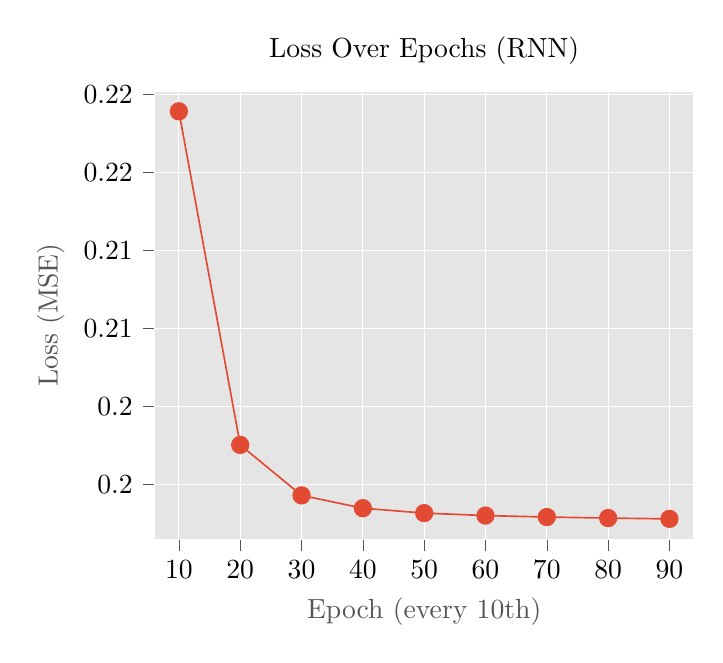
\begin{tikzpicture}

\definecolor{chocolate2267451}{RGB}{226,74,51}
\definecolor{dimgray85}{RGB}{85,85,85}
\definecolor{gainsboro229}{RGB}{229,229,229}

\begin{axis}[
axis background/.style={fill=gainsboro229},
axis line style={white},
tick align=outside,
tick pos=left,
title={Loss Over Epochs (RNN)},
x grid style={white},
xlabel=\textcolor{dimgray85}{Epoch (every 10th)},
xmajorgrids,
xmin=-0.4, xmax=8.4,
xtick style={color=dimgray85},
xtick={0,1,2,3,4,5,6,7,8},
xtick={0,1,2,3,4,5,6,7,8},
xticklabels={10,20,30,40,50,60,70,80,90},
xticklabels={10,20,30,40,50,60,70,80,90},
y grid style={white},
ylabel=\textcolor{dimgray85}{Loss (MSE)},
ymajorgrids,
ymin=0.191502721607685, ymax=0.220240204036236,
ytick style={color=dimgray85}
]
\addplot [semithick, chocolate2267451, mark=*, mark size=3, mark options={solid}]
table {%
0 0.218933954834938
1 0.197551742196083
2 0.194316670298576
3 0.193493545055389
4 0.193179294466972
5 0.193022191524506
6 0.192927539348602
7 0.19286160171032
8 0.192808970808983
};
\end{axis}

\end{tikzpicture}

  \caption{Simulation plot of the training error in MSE}
\end{figure}

\begin{figure}[H]
  \centering
    % This file was created with tikzplotlib v0.10.1.
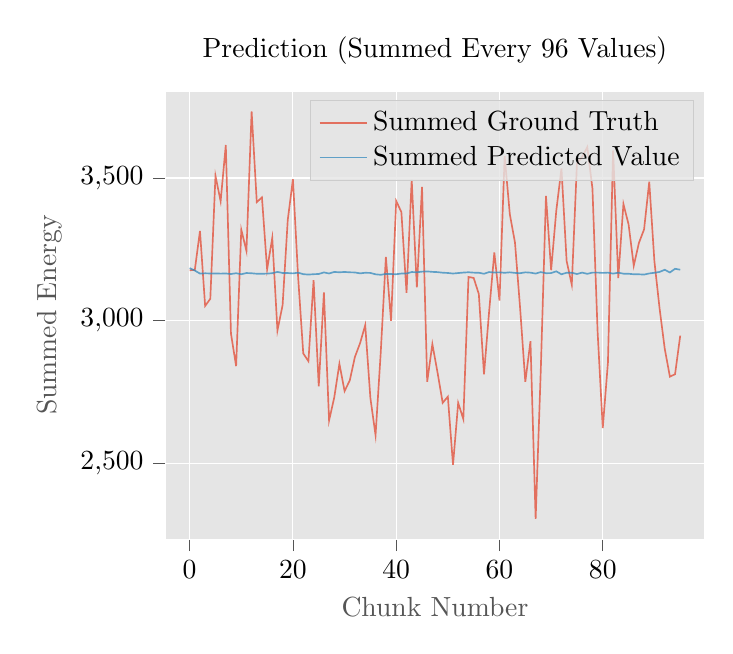
\begin{tikzpicture}

\definecolor{chocolate2267451}{RGB}{226,74,51}
\definecolor{dimgray85}{RGB}{85,85,85}
\definecolor{gainsboro229}{RGB}{229,229,229}
\definecolor{lightgray204}{RGB}{204,204,204}
\definecolor{steelblue52138189}{RGB}{52,138,189}

\begin{axis}[
axis background/.style={fill=gainsboro229},
axis line style={white},
legend cell align={left},
legend style={fill opacity=0.8, draw opacity=1, text opacity=1, draw=lightgray204, fill=gainsboro229},
tick align=outside,
tick pos=left,
title={Prediction (Summed Every 96 Values)},
x grid style={white},
xlabel=\textcolor{dimgray85}{Chunk Number},
xmajorgrids,
xmin=-4.75, xmax=99.75,
xtick style={color=dimgray85},
y grid style={white},
ylabel=\textcolor{dimgray85}{Summed Energy},
ymajorgrids,
ymin=2232.71514892578, ymax=3805.19818115234,
ytick style={color=dimgray85}
]
\addplot [semithick, chocolate2267451, opacity=0.75]
table {%
0 3176.2626953125
1 3177.3017578125
2 3314.248046875
3 3051.21997070312
4 3076.07666015625
5 3507.55541992188
6 3418.2587890625
7 3615.46606445312
8 2954.12255859375
9 2839.9013671875
10 3318.59375
11 3243.87353515625
12 3733.7216796875
13 3415.28759765625
14 3431.82641601562
15 3179.43579101562
16 3289.86547851562
17 2965.04077148438
18 3053.94287109375
19 3353.06591796875
20 3495.27685546875
21 3154.33618164062
22 2884.38427734375
23 2857.31982421875
24 3141.67114257812
25 2769.5673828125
26 3098.36474609375
27 2649.19067382812
28 2729.923828125
29 2848.14892578125
30 2752.65625
31 2789.24243164062
32 2872.119140625
33 2920.3779296875
34 2983.58227539062
35 2728.12939453125
36 2597.62133789062
37 2886.47021484375
38 3222.91259765625
39 2999.19873046875
40 3419.18969726562
41 3380.2451171875
42 3096.98950195312
43 3493.27001953125
44 3115.99462890625
45 3468.80517578125
46 2785.03881835938
47 2917.21142578125
48 2818.03759765625
49 2711.25634765625
50 2732.86328125
51 2493.6455078125
52 2711.1708984375
53 2654.22265625
54 3152.70654296875
55 3149.37768554688
56 3092.7509765625
57 2811.6884765625
58 3032.94799804688
59 3238.4306640625
60 3069.927734375
61 3576.82934570312
62 3372.86596679688
63 3273.59033203125
64 3042.29150390625
65 2784.796875
66 2927.5107421875
67 2304.19165039062
68 2828.05688476562
69 3436.94116210938
70 3176.529296875
71 3385.4111328125
72 3533.5458984375
73 3208.68408203125
74 3125.57763671875
75 3551.4072265625
76 3573.41088867188
77 3608.099609375
78 3463.40283203125
79 2960.390625
80 2622.99047851562
81 2852.43920898438
82 3596.98388671875
83 3149.06591796875
84 3408.431640625
85 3337.0126953125
86 3192.1865234375
87 3272.08227539062
88 3319.7421875
89 3486.60107421875
90 3207.33715820312
91 3042.77172851562
92 2900.98388671875
93 2803.02880859375
94 2811.72778320312
95 2946.9375
};
\addlegendentry{Summed Ground Truth}
\addplot [semithick, steelblue52138189, opacity=0.75]
table {%
0 3183.87890625
1 3175.28369140625
2 3164.5498046875
3 3165.60424804688
4 3164.923828125
5 3164.98876953125
6 3164.51611328125
7 3164.96655273438
8 3163.15795898438
9 3165.86181640625
10 3162.32763671875
11 3166.56274414062
12 3165.7265625
13 3163.98999023438
14 3164.03393554688
15 3164.490234375
16 3165.9833984375
17 3170.50341796875
18 3166.71118164062
19 3166.48193359375
20 3165.27490234375
21 3167.8583984375
22 3162.62060546875
23 3161.08544921875
24 3162.419921875
25 3163.21215820312
26 3168.7373046875
27 3164.9716796875
28 3170.33984375
29 3169.16015625
30 3170.26123046875
31 3169.0966796875
32 3168.5478515625
33 3165.3759765625
34 3167.5009765625
35 3166.88037109375
36 3162.06884765625
37 3160.36181640625
38 3163.37622070312
39 3162.95336914062
40 3162.37963867188
41 3164.73559570312
42 3164.81860351562
43 3170.10107421875
44 3169.15234375
45 3171.42700195312
46 3172.2119140625
47 3170.6240234375
48 3169.779296875
49 3167.6533203125
50 3166.7841796875
51 3164.783203125
52 3166.51220703125
53 3168.169921875
54 3169.28295898438
55 3167.86743164062
56 3167.43603515625
57 3164.0263671875
58 3169.92626953125
59 3168.40673828125
60 3168.97998046875
61 3167.37768554688
62 3169.02026367188
63 3167.0068359375
64 3165.97216796875
65 3169.02783203125
66 3167.83813476562
67 3164.646484375
68 3169.90869140625
69 3165.89013671875
70 3166.42846679688
71 3172.4638671875
72 3161.98852539062
73 3167.67333984375
74 3167.6884765625
75 3163.05737304688
76 3168.1181640625
77 3163.65087890625
78 3168.03662109375
79 3168.0888671875
80 3166.947265625
81 3167.96362304688
82 3164.4814453125
83 3167.810546875
84 3164.27319335938
85 3164.0400390625
86 3162.10302734375
87 3162.1171875
88 3161.0615234375
89 3165.10400390625
90 3167.4443359375
91 3170.43725585938
92 3177.94897460938
93 3168.56884765625
94 3181.4091796875
95 3178.17431640625
};
\addlegendentry{Summed Predicted Value}
\end{axis}

\end{tikzpicture}

  \caption{Simulation plot of the training error in MSE}
\end{figure}

I dunno mannnn

\begin{figure}[H]
  \centering
    % This file was created with tikzplotlib v0.10.1.
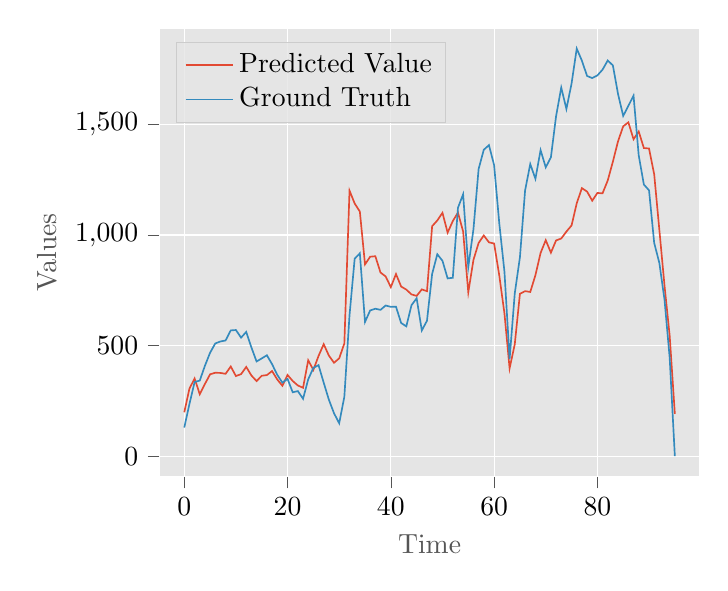
\begin{tikzpicture}

\definecolor{chocolate2267451}{RGB}{226,74,51}
\definecolor{dimgray85}{RGB}{85,85,85}
\definecolor{gainsboro229}{RGB}{229,229,229}
\definecolor{lightgray204}{RGB}{204,204,204}
\definecolor{steelblue52138189}{RGB}{52,138,189}

\begin{axis}[
axis background/.style={fill=gainsboro229},
axis line style={white},
legend cell align={left},
legend style={
  fill opacity=0.8,
  draw opacity=1,
  text opacity=1,
  at={(0.03,0.97)},
  anchor=north west,
  draw=lightgray204,
  fill=gainsboro229
},
tick align=outside,
tick pos=left,
x grid style={white},
xlabel=\textcolor{dimgray85}{Time},
xmajorgrids,
xmin=-4.75, xmax=99.75,
xtick style={color=dimgray85},
y grid style={white},
ylabel=\textcolor{dimgray85}{Values},
ymajorgrids,
ymin=-92.1626037597656, ymax=1935.41467895508,
ytick style={color=dimgray85}
]
\addplot [semithick, chocolate2267451]
table {%
0 198.435546875
1 305.348388671875
2 351.123596191406
3 280.257446289062
4 326.569091796875
5 370.180358886719
6 377.343719482422
7 376.40087890625
8 372.475738525391
9 405.539276123047
10 362.38134765625
11 370.920806884766
12 403.540588378906
13 364.933563232422
14 339.542297363281
15 363.637847900391
16 366.665252685547
17 384.902740478516
18 347.018432617188
19 318.433563232422
20 367.244812011719
21 339.870422363281
22 319.708190917969
23 309.245758056641
24 433.651580810547
25 390.149536132812
26 453.100219726562
27 506.504852294922
28 455.062927246094
29 422.359680175781
30 442.376708984375
31 509.964904785156
32 1200.81359863281
33 1142.65612792969
34 1106.35314941406
35 867.460571289062
36 901.951354980469
37 904.322814941406
38 830.587341308594
39 812.804077148438
40 764.389526367188
41 823.682739257812
42 767.180480957031
43 753.252502441406
44 731.552551269531
45 724.874206542969
46 754.290283203125
47 746.048278808594
48 1039.99963378906
49 1065.94799804688
50 1100.6025390625
51 1010.90161132812
52 1063.18933105469
53 1101.48229980469
54 1016.02459716797
55 741.026794433594
56 887.600708007812
57 964.327209472656
58 998.208618164062
59 967.022583007812
60 961.778259277344
61 817.461853027344
62 646.188659667969
63 396.981781005859
64 506.180969238281
65 734.420166015625
66 746.390686035156
67 742.519287109375
68 818.391174316406
69 919.016845703125
70 976.813232421875
71 920.355163574219
72 975.723083496094
73 984.385009765625
74 1015.71130371094
75 1043.39562988281
76 1143.63439941406
77 1212.20825195312
78 1196.73364257812
79 1155.51171875
80 1190.37890625
81 1188.79064941406
82 1246.54296875
83 1331.8662109375
84 1424.27600097656
85 1491.96276855469
86 1509.69458007812
87 1433.40051269531
88 1468.5234375
89 1393.54357910156
90 1391.48327636719
91 1275.0537109375
92 1023.29461669922
93 771.010620117188
94 544.187072753906
95 190.823638916016
};
\addlegendentry{Predicted Value}
\addplot [semithick, steelblue52138189]
table {%
0 129.466995239258
1 235.788040161133
2 335.239013671875
3 341.838958740234
4 408.933044433594
5 467.786010742188
6 509.720977783203
7 518.746948242188
8 523.286071777344
9 568.80615234375
10 570.518981933594
11 536.034057617188
12 561.9580078125
13 491.852081298828
14 428.232971191406
15 442.130004882812
16 456.27001953125
17 416.250061035156
18 367.885131835938
19 332.779968261719
20 349.243988037109
21 288.894012451172
22 294.340087890625
23 259.463012695312
24 347.286865234375
25 399.473541259766
26 411.618865966797
27 332.483306884766
28 255.468490600586
29 194.055541992188
30 148.838653564453
31 268.954803466797
32 637.510559082031
33 893.097900390625
34 917.37158203125
35 607.062194824219
36 659.185546875
37 666.920349121094
38 661.749267578125
39 681.366821289062
40 675.322570800781
41 675.73974609375
42 602.161743164062
43 586.995361328125
44 682.61181640625
45 713.9521484375
46 568.656127929688
47 612.405639648438
48 824.173767089844
49 913.189392089844
50 883.589294433594
51 803.853576660156
52 806.86767578125
53 1123.28039550781
54 1184.56921386719
55 855.762390136719
56 1026.18713378906
57 1298.71496582031
58 1385.69470214844
59 1406.73718261719
60 1316.287109375
61 1053.48266601562
62 835.051330566406
63 439.343688964844
64 735.6787109375
65 899.506713867188
66 1201.94165039062
67 1321.05944824219
68 1254.30261230469
69 1383.99926757812
70 1306.33471679688
71 1351.57092285156
72 1537.50439453125
73 1666.82348632812
74 1570.27392578125
75 1685.42407226562
76 1843.25207519531
77 1788.52404785156
78 1719.50329589844
79 1709.91394042969
80 1721.95104980469
81 1748.08654785156
82 1789.38952636719
83 1767.27990722656
84 1637.69860839844
85 1538.72326660156
86 1584.41137695312
87 1630.5771484375
88 1360.75805664062
89 1228.44470214844
90 1202.36315917969
91 964.465759277344
92 873.629699707031
93 707.248962402344
94 444.571258544922
95 0
};
\addlegendentry{Ground Truth}
\end{axis}

\end{tikzpicture}

  \caption{Simulation plot comparing the predicted value with the ground truth}
\end{figure}


%Is the federated learning efficient in this scenario of appliance energy consumption prediction? Please discuss whether the performance of model training can be improved by adding more epochs or through other configuration changes.


\section{Prediction with LSTM}

The following models use the same configurations as the previous model, except the trainer uses LSTM instead of regular RNN.

\begin{figure}[H]
  \centering
    % This file was created with tikzplotlib v0.10.1.
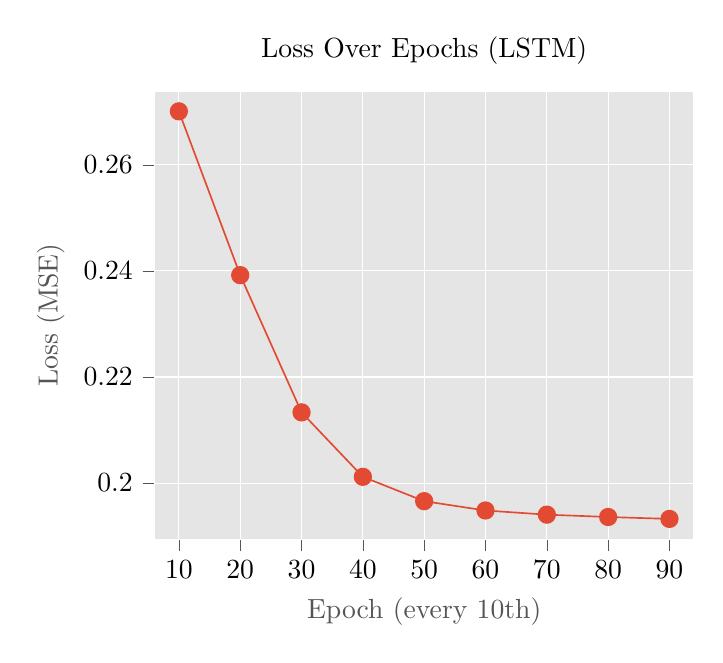
\begin{tikzpicture}

\definecolor{chocolate2267451}{RGB}{226,74,51}
\definecolor{dimgray85}{RGB}{85,85,85}
\definecolor{gainsboro229}{RGB}{229,229,229}

\begin{axis}[
axis background/.style={fill=gainsboro229},
axis line style={white},
tick align=outside,
tick pos=left,
title={Loss Over Epochs (LSTM)},
x grid style={white},
xlabel=\textcolor{dimgray85}{Epoch (every 10th)},
xmajorgrids,
xmin=-0.4, xmax=8.4,
xtick style={color=dimgray85},
xtick={0,1,2,3,4,5,6,7,8},
xtick={0,1,2,3,4,5,6,7,8},
xticklabels={10,20,30,40,50,60,70,80,90},
xticklabels={10,20,30,40,50,60,70,80,90},
y grid style={white},
ylabel=\textcolor{dimgray85}{Loss (MSE)},
ymajorgrids,
ymin=0.189402960240841, ymax=0.273933596909046,
ytick style={color=dimgray85}
]
\addplot [semithick, chocolate2267451, mark=*, mark size=3, mark options={solid}]
table {%
0 0.27009129524231
1 0.239204823970795
2 0.21332985162735
3 0.201177880167961
4 0.196588724851608
5 0.194829702377319
6 0.194046154618263
7 0.193602621555328
8 0.193245261907578
};
\end{axis}

\end{tikzpicture}

  \caption{Simulation plot of the training error in MSE}
\end{figure}


\begin{figure}[H]
  \centering
    \input{report/figures/pred-lstm-test}
  \caption{Simulation plot comparing the predicted value with the ground truth}
\end{figure}

 %Compare the performance with that of RNN regarding execution time and prediction error during the test.

\chapter{Classifying Appliance Types}

This section reports the results of the classification model: determining the types of application based on the daily consumption of an appliance.

\section{Classification using Regular RNN}

%Is the federated learning efficient in this scenario of appliance classification? Please use simulation plots to show the classification accuracy during the training process using training (or training and validation) data, and show the classification accuracy of the trained model using test data. Please discuss whether the accuracy during the training and testing can be improved by adding more epochs or through other configuration changes.

\section{Confusion Matrix}

%The accuracy in Question 2.1 manifests how the model works for all the appliance as a whole.You also need to show how the classification works for each appliance. To do so, you need to generate the confusion matrix of the classification result, both for the model training and testing. The confusion matrix should present the classification accuracy for each appliance.

\section{Classification using LSTM}

%Keep the same settings as in Question 2.1 and 2.2, except that you use LSTM when implementing federated learning. You then show the simulation plots as required in Question 2.1 and 2.2, and compare with the results when using RNN.

\chapter{Conclusion}

In conclusion, Why is it so hard to make intuitive code that just works?? Google, you're a multi-billion dollar company.. please! 
\newpage

\nocite{tensorflow2015-whitepaper}
\nocite{dataset}

\printbibliography{}

\vspace*{10mm}
\end{document}